\section{MTU Discovery}
\label{sec:MTU Discovery}

\subsection{Einleitung}
Mithilfe der \acs{MTU} (Maximum Transmission Unit) wird festgelegt wie gross ein Netzwerkpaket maximal sein darf, so dass es nicht in mehrere Pakete aufgeteilt werden muss. Wenn die \acs{MTU} korrekt bestimmt wurde dann wird Paket-Fragmentierung verhindert und die Performance der Netzwerkverbindung ist deutlich besser. 

Normalerweise wird die \acs{MTU} automatisch via \acs{PMTUD} (Path MTU Discovery) ermittelt. Dabei werden \acs{ICMP} Pakete unterschiedlicher Grösse die mit einem "Don't fragment" Flag versehen sind über die Verbindung gesandt. Wenn ein solches Paket auf ein Netzwerkgerät trifft dass eine kleinere \acs{MTU} konfiguriert hat als die Paketgrösse wird das Paket nicht weitergesendet, stattdessen wird ein \acs{ICMP} Paket mit dem Inhalt "Fragmentation needed" retourniert. So weiss der \acs{PMTUD} Algorithmus dass die \acs{MTU} der Verbindung überschritten wurde.

\acs{PMTUD} hat jedoch ein Problem. Router die, die \acs{ICMP} Pakete weiterleiten oder aber ein "Fragmentation needed" Paket zurücksenden sollten tun dies nicht immer. Dieses Fehlverhalten gibt es aus mehreren Gründen. Zum einen wegen Kernel-Bugs, Fehlkonfigurationen und zum anderen auch weil Firewalls manchmal so konfiguriert werden dass sie \acs{ICMP} Nachrichten nicht durchlassen auf Grund von Sicherheitsbedenken.

Da man sich also nicht auf \acs{PMTUD} verlassen kann um die \acs{MTU} einer Verbindung festzustellen wird mit dieser Arbeit eine \acs{MTU} Discovery implementiert die innerhalb einer \acs{IPSec} \acs{VPN} Verbindung durchgeführt werden kann.

%http://en.wikipedia.org/wiki/Path_MTU_Discovery
%http://tools.ietf.org/html/rfc2923
\todo{Citation needed}

\subsection{Path MTU Discovery}
Die Path MTU Discovery \acs{PMTUD} ist eine standardisierte Technik um die \acs{MTU} festzustellen.  Bei \acs{IPv4} funktioniert \acs{PMTUD} folgendermassen: Es werden \acs{ICMP} Pakete unterschiedlicher Grösse über die Netzwerkverbindung gesendet. Geräte deren \acs{MTU} kleiner als die Grösse des versendeten Pakets ist verwerfen das Paket und senden stattdessen eine \acs{ICMP} Nachricht mit dem Inhalt "Fragmentation Needed" zurück. So weiss der \acs{PMTUD} Algorithmus dass die versendeten Pakete noch zu gross sind um ihr Ziel zu erreichen. Die versendeten Pakete werden also verkleinert, und der Prozess wiederholt, bis eine Übertragungsgrösse gefunden wird mit der ein Paket den ganzen Pfad ohne Fragmentierung traversieren kann.

Doch wie bereits in der Einleitung angesprochen gibt es bei \acs{PMTUD} ein Problem. Viele Netzwerk-Sicherheit Geräte blockieren \acs{ICMP} Nachrichten. Dies beinhaltet die Errors "Fragmentation Needed" des \acs{PMTUD} Algorithmus. Bei der \osag wurde eben dieses Problem auch beobachtet, so gibt es \acs{VPN} Tunnels die über schlecht konfigurierte Router von Dritten laufen und so mit

%http://en.wikipedia.org/wiki/Path_MTU_Discovery
\todo{Citation needed}

\subsection{MTU-Bestimmung - Idee}
Um das Problem der blockierten \acs{ICMP} Packeten zu vermeiden bestimmt das \tool die \acs{MTU} innerhalb des \acs{VPN} Tunnels. Gegenüber den Routern die normalerweise die \acs{ICMP} Pakete blockieren würden sehen die Pakete des \tool wie normale \acs{IPSec} \acs{ESP}s aus. Sie haben jedoch wie auch die \acs{ICMP} Pakete von \acs{PMTUD} den "Don't Fragment" Flag gesetzt. Dadurch wird verhindert das die Pakete automatisch fragmentiert werden wenn sie die \acs{MTU} eines Geräts überschreiten. Im Gegensatz zu \acs{PMTUD} kann man hier nicht auf ein \acs{ICMP} "Fragmentation Needed" Paket zählen das von einer Netzwerkkomponente beim überschreiten der \acs{MTU} versendet wird. Pakete die, die \acs{MTU} überschreiben werden einfach verworfen. Deshalb muss das \tool auf beiden Seiten des \acs{VPN} Tunnels laufen und Pakete die ankommen beantworten.

Innerhalb des Tunnels wird wie bei \acs{PMTUD} auf \acs{ICMP} Pakete gesetzt. Die vom \tool versendeten Pakete enthalten eine Payload die aus den folgenden Angaben besteht:

\begin{itemize}
  \item \textbf{AppID:} Eindeutige ID des aktiven \tool. Wird verwendet um mehrere gleichzeitig laufende \tool auf einem Rechner zu unterscheiden.
  \item \textbf{ChannelID:} ID des GO-Channels von dem das Paket versendet wurde. Wird benötigt um für mehrere Tunnels gleichzeitig die \acs{MTU} festzustellen zu können.
  \item \textbf{Command:} Die eigentliche Nachricht des Pakets. z.B. "MTU?" als Request oder "OK" als Antwort.
  \item \textbf{Null-Array:} Ein mit Nullen gefülltes Array von variabler Grösse. Wird verwendet um dem Paket seine vorbestimmte Grösse zu geben.
\end{itemize}

% GFX Trim left bottom right top
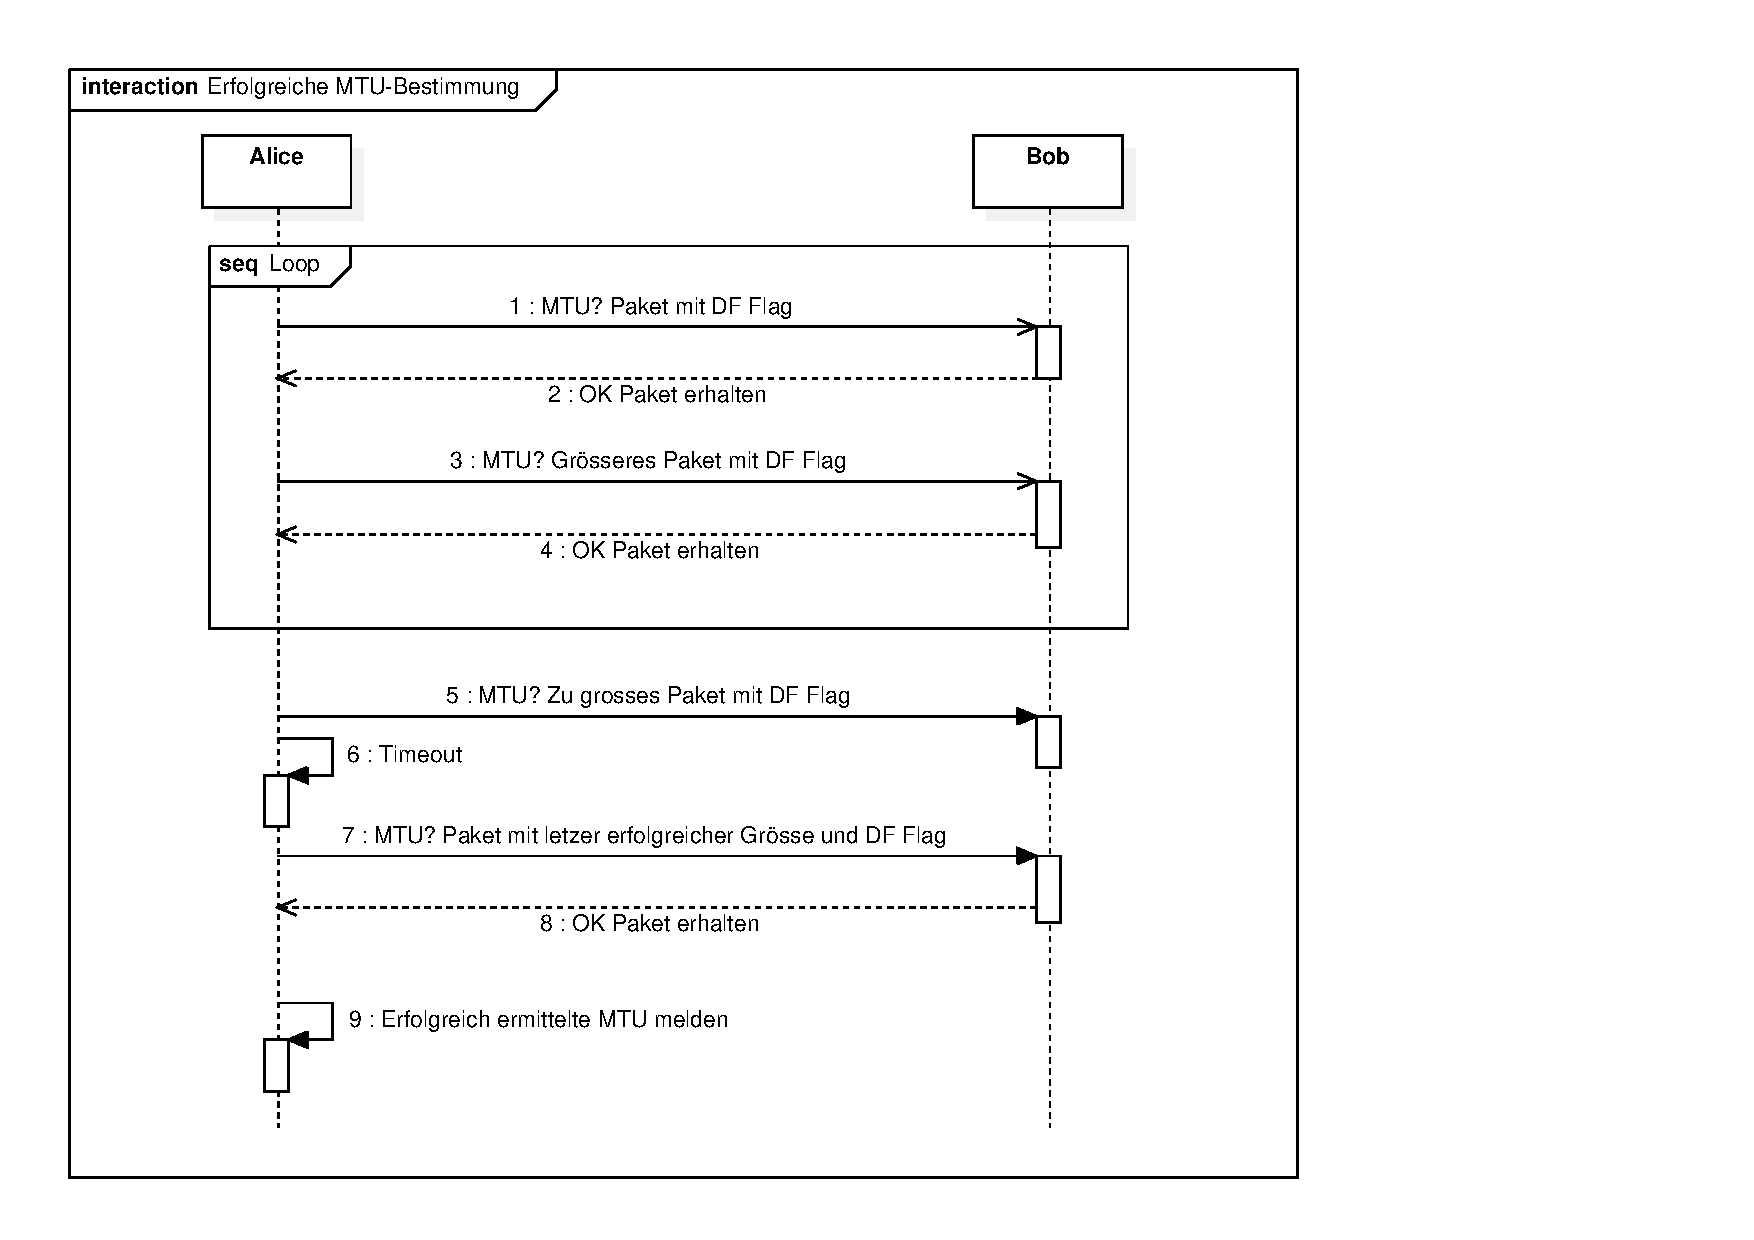
\includegraphics[trim=10 10 200 10,clip,width=\textwidth]{mainpart/implementation/img/MTUBestimmungErfolgreich}

Die obenstehende Grafik zeigt den weiteren Ablauf der \acs{MTU} Bestimmung mit dem \tool. Alice sendet ein Paket mit dem Command "MTU?" und einer bestimmten Grösse an Bob. Wenn Bob das Paket erhält, sendet er "OK als Antwort. Alice erhöht darauf die Paketgrösse und fragt Bob erneut mit "MTU?" an. Dies wird so lange wiederholt bis das Paket nicht mehr ankommt. Bob erhält also das "MTU?" Paket nicht und kann somit Alice auch keine Antwort schicken. Alice hat jedoch ein Timeout Timer und nach einer vordefinierten Zeit ohne Antwort geht Alice davon aus dass das Paket nicht angekommen ist. Alice sendet nun ein Paket mit der letzten erfolgreichen Grösse um sicher zu Stellen das die Netzwerkverbindung selbst noch besteht und protokolliert dann die letzte erfolgreiche \acs{MTU}.

\subsection{MTU-Bestimmung - FastMTU}
Die im oberen Abschnitt beschrieben Art der \acs{MTU} Bestimmung war gut als ein erster Schritt im iterativen Softwareentwicklungsprozess. Für einen produktiven Betrieb wäre sie aber nicht zu gebrauchen. Zum einen ist die oben beschriebene Variante nur exakt wenn man einen Vergösserungs-Schritt von einem Byte nimmt und wodurch der Algorithmus aber sehr langsam wird. Und zum anderen ist sie auch Anfällig auf Paket-Verluste.
Daher wurde der Algorithmus nach der ersten Iteration erweitert und überarbeitet. Die neue Variante wird von uns liebevoll "FastMTU" genannt.

Bei der FastMTU Bestimmung bleibt das grundlegende Prinzip gleich, es werden Pakete unterschiedlicher Grösse versendet so dass man herausfinden kann welche ankommen und welche verworfen werden. Neu wird jedoch nicht nur ein Paket aufs Mal versendet sondert einen ganze Batch von Paketen. Dazu wird aus der Konfiguration einen sogenannten Range ausgelesen. Der Range besteht aus zwei Byte-Grössen die festlegen worin sich die \acs{MTU} typischerweise befinden sollte. Zum Beispiel zwischen 0 und 2000 Bytes. Dann wird aus der Konfiguration ausgelesen wie viele Pakete aufs Mal versendet werden sollen. Mehr gleichzeitige Pakete führen zu einer schnelleren Bestimmung der \acs{MTU}, haben aber auch zur folge dass die Verbindung stärker belastet wird und so möglicherweise wichtiger Kunden-Traffic ausgebremst wird. Als Default-Wert gehen wir von 20 gleichzeitigen Paketen aus. Der Range 0-2000 Bytes wird jetzt also durch 20 geteilt. Damit erhält man 20 Pakete die sich je um 100 Bytes unterscheiden. Diese 20 Pakete werden nun als einen Batch versendet.
Für alle Pakete die auf der anderen Seite des Tunnels ankommen wird nun eine Antwort generiert. Bei einer MTU von 1500 Bytes würden die ersten 15 Pakete ankommen. Der Sender weiss jetzt also dass die exakte \acs{MTU} zwischen dem letzten erfolgreichen Paket (1500) und dem ersten nicht erfolgreichen Paket (1600) sein muss. 1500-1600 Bytes wird nun als nun als neuer Range gesetzt und erneut durch die Anzahl gleichzeitiger Pakete geteilt. Die Pakete des zweiten Batches haben also noch 5 Byte Unterschied. Dieser Vorgang wird so lange wiederholt bis der Unterschied zwischen den Paketen eines Batches nur noch 1 Byte sind. Jetzt weiss man das man die exakte \acs{MTU} gefunden hat.

Mit FastMTU weiss man also bereits im vorraus wie lange das Finden der exakten \acs{MTU} dauern wird. Bei einer MTU zwischen 0-2000 Bytes werden 3 Batches an Paketen versendet. Pro Batch muss jeweils die Dauer des Timeout-Timers gewartet werden. Gemäss der \osag ist ein Timeout von 10 Sekunden realistisch. Daher hätte das Bestimmen diese \acs{MTU} 30Sekunden gedauert.
Die verbrauchte Zeit beim Bestimmen von FastMTU lässt sich sehr leicht via der Konfiguration optimieren. So hat man die Möglichkeit den Range stärker einzuschränken, den Timeout zu verkürzen oder aber mehr Pakete pro Batch zu versenden.

\todo{Grafik die FastMTU zeigt.}

Auch wenn die \acs{MTU} sich ausserhalb des Ranges befindet wird sie von FastMTU noch korrekt detektiert. Wenn nämlich alle Pakete eines Batches eine erfolgreiche Antwort der Gegenseite generieren, dann wird der nächste Range einfach um die Grösse des überprüften Range vergrössert. Im Beispiel mit einem Range von 0-2000 Bytes würde jetzt einfach 2000-4000 Bytes überprüft.